\documentclass[11pt]{article}

\usepackage[a4paper,margin=1in]{geometry}
\usepackage[T1]{fontenc}
\usepackage{amsmath,amssymb}
\usepackage{graphicx}
\usepackage{booktabs}
\usepackage{caption}
\usepackage{xcolor}
\usepackage{listings}
\usepackage[section]{placeins}
\usepackage[hidelinks]{hyperref}

\renewcommand{\topfraction}{0.9}
\renewcommand{\bottomfraction}{0.8}
\renewcommand{\textfraction}{0.07}
\renewcommand{\floatpagefraction}{0.75}
\setcounter{topnumber}{3}
\setcounter{totalnumber}{5}

\captionsetup{font=small,labelfont=bf}
\graphicspath{{figures/}}
\definecolor{ink2}{HTML}{52514E}
\lstset{basicstyle=\ttfamily\scriptsize,columns=fullflexible,breaklines=true,
        commentstyle=\color{ink2},frame=lines,numbers=left,numberstyle=\tiny\color{ink2}}

\newcommand{\E}{\mathbb{E}}
\newcommand{\Var}{\mathrm{Var}}
\newcommand{\QVFinest}{0.997}
\newcommand{\TVFinest}{204}
\newcommand{\GBMMeanTh}{108.33}
\newcommand{\GBMMedTh}{105.00}
\newcommand{\GBMMin}{39.8}
\newcommand{\GBMMax}{273.6}
\newcommand{\EulerOrder}{0.49}
\newcommand{\MilsteinOrder}{0.99}
\newcommand{\OUHalfLife}{0.35}
\newcommand{\CIRSigma}{0.0894}
\newcommand{\FellerLHS}{0.050}
\newcommand{\FellerRHS}{0.0080}
\newcommand{\PNegTh}{0.64}
\newcommand{\PNegSim}{0.57}
\newcommand{\PNegEver}{25.8}
\newcommand{\CIRMin}{0.159}
\newcommand{\VasMin}{-5.26}
\newcommand{\YInf}{4.92}
\newcommand{\MaxZ}{1.86}
\newcommand{\NChecks}{19}


\title{Simulating Brownian Motion, Geometric Brownian Motion,\\
the Ornstein--Uhlenbeck Process and Short-Rate Models}
\author{Aaryan Pradhan (22CH3FP25)\\[6pt]
\small MA30247 Financial Mathematics, Individual Project\\
\small Indian Institute of Technology Kharagpur}
\date{November 2026}

\begin{document}
\maketitle

\begin{abstract}
\noindent We simulate the processes set for this project: Brownian motion, geometric Brownian
motion, the Ornstein--Uhlenbeck process and the short-rate (VIR) model. For the short rate we
run two models, Vasicek and Cox--Ingersoll--Ross (CIR). Every process is drawn from its exact
transition law, so the only error left is Monte Carlo noise. With 20{,}000 paths, all \NChecks{}
simulated moments, probabilities and bond prices lie within \MaxZ{} standard errors of their
closed-form values. The plots show how each model behaves. The variance of Brownian motion grows
linearly in time. Geometric Brownian motion is lognormal, and its median falls further below its
mean as volatility rises. The Ornstein--Uhlenbeck process forgets its starting point with a
half-life of $\ln 2/\theta$. The Vasicek rate goes below zero on \PNegEver\% of paths within ten
years, while a CIR rate with the same mean and long-run variance never does. Finally, we measure
the strong error of the Euler and Milstein schemes for geometric Brownian motion and find orders
\EulerOrder{} and \MilsteinOrder, close to the theoretical $1/2$ and $1$.
\end{abstract}

\noindent\textbf{\textit{Keywords:}} Brownian motion; Geometric Brownian motion;
Ornstein--Uhlenbeck process; Vasicek model; CIR model; Exact simulation; Monte Carlo

%=====================================================================
\section{Introduction}

Most models in mathematical finance are stochastic differential equations (SDEs). A stock price,
an interest rate or a spread is written as a drift term plus a noise term, and the noise comes
from Brownian motion. A few of these models can be solved by hand. For the others, and for any
payoff that depends on the whole path, we simulate.

This report simulates the processes listed in the project brief. Brownian motion is the noise
source for all of them. Geometric Brownian motion (GBM) is the stock price model behind
Samuelson~\cite{samuelson1965} and Black and Scholes~\cite{black1973}. The Ornstein--Uhlenbeck
(OU) process~\cite{uhlenbeck1930} adds a pull toward a long-run level. Vasicek~\cite{vasicek1977}
used the OU process as a model of the short interest rate. The brief calls the short-rate model
``VIR''. We read this as the Vasicek interest-rate model, and since the same abbreviation is
sometimes used for the Cox--Ingersoll--Ross (CIR) model~\cite{cox1985}, we simulate both. The
two differ in a single term, and that difference decides whether rates can turn negative.

Each of these models has a known solution, and we use it twice. First, we simulate from it:
each time step is drawn from the exact conditional distribution, so there is no discretization
error in the paths~\cite{glasserman2003}. Second, we check against it: every simulated mean,
variance, probability and bond price is compared with its formula, measured in units of its
Monte Carlo standard error.

Section~\ref{sec:models} states the models and their solutions. Section~\ref{sec:method}
describes the simulation. Section~\ref{sec:results} goes through the results one process at a
time, and Section~\ref{sec:conclusion} concludes. The code in the appendix rebuilds every
figure and number in this report in a few seconds. Figure~\ref{fig:overview} shows one path of
each process.

\begin{figure}[h]
\centering
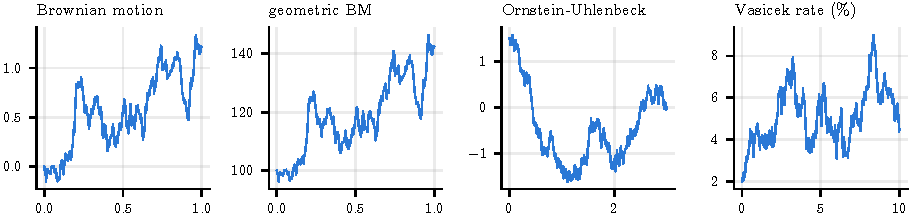
\includegraphics[width=\textwidth]{overview}
\caption{One simulated path of each process. Parameters are in Table~\ref{tab:params}.
Brownian motion and GBM wander off with no level to return to; the OU process and the Vasicek
rate are pulled back toward their long-run levels ($0$ and $5\%$).}
\label{fig:overview}
\end{figure}

%=====================================================================
\section{The models}
\label{sec:models}

Throughout, $(W_t)_{t\ge0}$ is a standard Brownian motion and $Z$ is a standard normal random
variable. Table~\ref{tab:models} at the end of the section collects the results.

\subsection{Brownian motion}

A standard Brownian motion has $W_0=0$, continuous paths, and independent increments with
\begin{equation}
W_t-W_s\sim N(0,\,t-s), \qquad 0\le s<t.
\label{eq:bm}
\end{equation}
So $\E[W_t]=0$, $\Var[W_t]=t$ and $\mathrm{Cov}(W_s,W_t)=\min(s,t)$. The spread of $W_t$ grows
like $\sqrt t$, not like $t$.

Two path properties matter for what follows. Take a partition $0=t_0<t_1<\dots<t_n=T$ whose
largest step goes to zero. Then the \emph{quadratic variation} $\sum_k (W_{t_{k+1}}-W_{t_k})^2$
converges to $T$, while the total variation $\sum_k |W_{t_{k+1}}-W_{t_k}|$ goes to infinity.
A Brownian path is too rough for ordinary calculus. The finite quadratic variation is the source
of the extra $\tfrac12 f''$ term in It\^o's formula~\cite{shreve2004}.

\subsection{Geometric Brownian motion}

A stock price with expected return $\mu$ and volatility $\sigma$ follows
\begin{equation}
dS_t=\mu S_t\,dt+\sigma S_t\,dW_t, \qquad S_0>0.
\label{eq:gbm}
\end{equation}
It\^o's formula applied to $\ln S_t$ gives $d\ln S_t=(\mu-\tfrac12\sigma^2)\,dt+\sigma\,dW_t$.
The right side has constant coefficients, so we can integrate it directly:
\begin{equation}
S_t=S_0\exp\!\Big(\big(\mu-\tfrac12\sigma^2\big)t+\sigma W_t\Big).
\label{eq:gbmsol}
\end{equation}
Hence $\ln S_t$ is normal and $S_t$ is lognormal. It is always positive, and
\begin{equation}
\E[S_t]=S_0e^{\mu t},\qquad
\mathrm{median}(S_t)=S_0e^{(\mu-\sigma^2/2)t},\qquad
\Var[S_t]=S_0^2e^{2\mu t}\big(e^{\sigma^2t}-1\big).
\end{equation}
The mean is larger than the median by the factor $e^{\sigma^2t/2}$. A few very good paths pull
the mean up, while most paths end below it.

\subsection{The Ornstein--Uhlenbeck process}

The OU process is pulled toward a level $\mu$ at speed $\theta>0$:
\begin{equation}
dX_t=\theta(\mu-X_t)\,dt+\sigma\,dW_t.
\label{eq:ou}
\end{equation}
Multiply by $e^{\theta t}$. It\^o's product rule gives
$d(e^{\theta t}X_t)=\theta\mu e^{\theta t}\,dt+\sigma e^{\theta t}\,dW_t$, and integrating
from $0$ to $t$,
\begin{equation}
X_t=\mu+(X_0-\mu)e^{-\theta t}+\sigma\int_0^t e^{-\theta(t-s)}\,dW_s.
\label{eq:ousol}
\end{equation}
The stochastic integral has a deterministic integrand, so it is normal with mean zero. By the
It\^o isometry its variance is $\sigma^2\!\int_0^t e^{-2\theta(t-s)}ds$. Therefore
\begin{equation}
\E[X_t]=\mu+(X_0-\mu)e^{-\theta t},\qquad
\Var[X_t]=\frac{\sigma^2}{2\theta}\big(1-e^{-2\theta t}\big).
\label{eq:oumom}
\end{equation}
As $t\to\infty$ the law of $X_t$ tends to $N(\mu,\sigma^2/2\theta)$, the \emph{stationary}
distribution. The expected distance to $\mu$ halves every $\ln2/\theta$ units of time. If $X_0$ is drawn
from the stationary law, then $\mathrm{corr}(X_s,X_{s+\tau})=e^{-\theta\tau}$.

\subsection{Short-rate models (VIR): Vasicek and CIR}

Let $r_t$ be the instantaneous short interest rate. Vasicek~\cite{vasicek1977} takes
\begin{equation}
dr_t=a(b-r_t)\,dt+\sigma\,dW_t ,
\label{eq:vas}
\end{equation}
which is \eqref{eq:ou} with $\theta=a$ and $\mu=b$. So $r_t$ is normal with mean
$b+(r_0-b)e^{-at}$ and variance $\frac{\sigma^2}{2a}(1-e^{-2at})$. A normal variable can be
negative, so $\mathbb P(r_t<0)=\Phi\big(-\E[r_t]/\sqrt{\Var[r_t]}\big)>0$ for every $t>0$.

The price at time 0 of a zero-coupon bond paying 1 at time $T$ is
$P(0,T)=\E\big[\exp(-\int_0^T r_s\,ds)\big]$, where we treat \eqref{eq:vas} as the
risk-neutral dynamics. For Vasicek this expectation has the closed form
\begin{equation}
P(0,T)=A(T)e^{-B(T)r_0},\quad
B(T)=\frac{1-e^{-aT}}{a},\quad
\ln A(T)=\Big(b-\frac{\sigma^2}{2a^2}\Big)\big(B(T)-T\big)-\frac{\sigma^2B(T)^2}{4a}.
\label{eq:vasbond}
\end{equation}
The yield $y(0,T)=-\ln P(0,T)/T$ tends to $b-\sigma^2/(2a^2)$ as $T\to\infty$.

The CIR model~\cite{cox1985} multiplies the noise by $\sqrt{r_t}$:
\begin{equation}
dr_t=a(b-r_t)\,dt+\sigma\sqrt{r_t}\,dW_t .
\label{eq:cir}
\end{equation}
As $r_t$ approaches zero the noise dies out and the drift $ab>0$ pushes the rate back up. If the
Feller condition $2ab\ge\sigma^2$ holds, the rate never reaches zero. The mean is the same as in
Vasicek. The variance is
$r_0\frac{\sigma^2}{a}(e^{-at}-e^{-2at})+\frac{b\sigma^2}{2a}(1-e^{-at})^2$, and
$r_t$ is a scaled noncentral chi-square variable (Section~\ref{sec:method}). The CIR bond price
also has the form $A(T)e^{-B(T)r_0}$, now with $h=\sqrt{a^2+2\sigma^2}$,
\begin{equation}
B(T)=\frac{2(e^{hT}-1)}{(h+a)(e^{hT}-1)+2h},\qquad
A(T)=\left(\frac{2h\,e^{(a+h)T/2}}{(h+a)(e^{hT}-1)+2h}\right)^{2ab/\sigma^2}.
\label{eq:cirbond}
\end{equation}

\begin{table}[h]
\centering\small
\caption{The models at a glance.}
\label{tab:models}
\begin{tabular}{@{}lllll@{}}
\toprule
Model & SDE & Law of $X_t$ & $\E[X_t]$ & Values \\
\midrule
BM      & $dW_t$                               & normal            & $0$                       & $\mathbb R$ \\
GBM     & $\mu S\,dt+\sigma S\,dW$             & lognormal         & $S_0e^{\mu t}$            & $(0,\infty)$ \\
OU      & $\theta(\mu-X)\,dt+\sigma\,dW$       & normal            & $\mu+(X_0-\mu)e^{-\theta t}$ & $\mathbb R$ \\
Vasicek & $a(b-r)\,dt+\sigma\,dW$              & normal            & $b+(r_0-b)e^{-at}$        & $\mathbb R$ \\
CIR     & $a(b-r)\,dt+\sigma\sqrt r\,dW$       & scaled $\chi'^2$  & $b+(r_0-b)e^{-at}$        & $(0,\infty)$ if $2ab\ge\sigma^2$ \\
\bottomrule
\end{tabular}
\end{table}

%=====================================================================
\section{Simulation method}
\label{sec:method}

We use an equally spaced grid $t_k=k\,\Delta t$ and independent draws $Z_k\sim N(0,1)$. Each
update below is the exact conditional law of the next value given the current one, so the
simulated values on the grid have exactly the right joint distribution~\cite{glasserman2003}:
\begin{align}
\text{BM:}\quad & W_{k+1}=W_k+\sqrt{\Delta t}\,Z_k, \\
\text{GBM:}\quad & S_{k+1}=S_k\exp\!\big((\mu-\tfrac12\sigma^2)\Delta t+\sigma\sqrt{\Delta t}\,Z_k\big), \\
\text{OU, Vasicek:}\quad & X_{k+1}=\mu+(X_k-\mu)e^{-\theta\Delta t}
   +\sigma\sqrt{\tfrac{1-e^{-2\theta\Delta t}}{2\theta}}\;Z_k, \label{eq:ouexact}\\
\text{CIR:}\quad & r_{k+1}=c\,\chi'^2_\nu(\lambda_k),\quad
   c=\tfrac{\sigma^2(1-e^{-a\Delta t})}{4a},\ \nu=\tfrac{4ab}{\sigma^2},\
   \lambda_k=\tfrac{r_ke^{-a\Delta t}}{c}. \label{eq:cirexact}
\end{align}
Here $\chi'^2_\nu(\lambda)$ is a noncentral chi-square draw with $\nu$ degrees of freedom and
noncentrality $\lambda$. GBM is computed from \eqref{eq:gbmsol} on the same Brownian paths, which
is the same thing as the GBM update above. For bond prices we need $\int_0^T r_s\,ds$ on each
path, which we approximate with the trapezoid rule. This is the only discretization error in the
study, and Table~\ref{tab:moments} shows it is smaller than the Monte Carlo noise.

\paragraph{Euler and Milstein.} To see what exact simulation saves, we also run the two standard
schemes on GBM~\cite{kloeden1992,higham2001}, with $\Delta W_k=\sqrt{\Delta t}\,Z_k$:
\begin{align}
\text{Euler--Maruyama:}\quad & S_{k+1}=S_k+\mu S_k\Delta t+\sigma S_k\Delta W_k, \\
\text{Milstein:}\quad & S_{k+1}=S_k+\mu S_k\Delta t+\sigma S_k\Delta W_k
   +\tfrac12\sigma^2S_k\big(\Delta W_k^2-\Delta t\big).
\end{align}
We drive both with the same Brownian increments as the exact solution and measure the strong
error $\E\big|S_T^{\Delta t}-S_T\big|$. Theory says it shrinks like $\Delta t^{1/2}$ for Euler and
like $\Delta t$ for Milstein.

\paragraph{Checking against theory.} For a quantity $\E[f]$ we report the sample mean
$\hat m$ of $f$ over $M$ paths, its standard error $\hat s/\sqrt M$, and
$z=(\hat m-\text{theory})/(\hat s/\sqrt M)$. If the code is correct, $z$ is roughly standard
normal. A variance is checked as the mean of $(X-\E X)^2$, a probability as the mean of an
indicator and a bond price as the mean of $e^{-\int r}$. The code stops if any $|z|$ exceeds 4.

\begin{table}[h]
\centering\small
\caption{Parameters. All runs use $M=20{,}000$ paths and the PCG64 generator with seed 2026.}
\label{tab:params}
\begin{tabular}{@{}llll@{}}
\toprule
Process & Parameters & Horizon & Step \\
\midrule
BM      & $W_0=0$                                                   & $T=1$  & $\Delta t=1/252$ (daily) \\
GBM     & $S_0=100$, $\mu=0.08$, $\sigma=0.25$                      & $T=1$  & $1/252$ \\
OU      & $X_0=1.5$, $\theta=2$, $\mu=0$, $\sigma=1$                & $T=3$  & $1/200$ \\
Vasicek & $r_0=2\%$, $a=0.5$, $b=5\%$, $\sigma=0.02$                & $T=10$ & $1/52$ (weekly) \\
CIR     & $r_0=2\%$, $a=0.5$, $b=5\%$, $\sigma=\CIRSigma$            & $T=10$ & $1/52$ \\
\bottomrule
\end{tabular}
\end{table}

The CIR volatility is set to $\sigma_{\text{CIR}}=\sigma_{\text{Vas}}/\sqrt b$. With this choice
both rate models have the same mean at every date and the same long-run variance,
$\sigma_{\text{Vas}}^2/2a$, so any difference between them comes from the shape of the noise.
The Feller condition holds: $2ab=\FellerLHS\ge\sigma_{\text{CIR}}^2=\FellerRHS$.

%=====================================================================
\section{Results}
\label{sec:results}

\subsection{Brownian motion}

Figure~\ref{fig:bmpaths} shows ten paths with the 50\% and 90\% bands of all 20{,}000. The bands
open like $\sqrt t$. The outer band lies just inside the $\pm2\sqrt t$ curves, at $\pm1.645\sqrt t$,
because $W_t$ is $N(0,t)$ and 90\% of a normal law lies within $1.645$ standard deviations.

\begin{figure}[h]
\centering
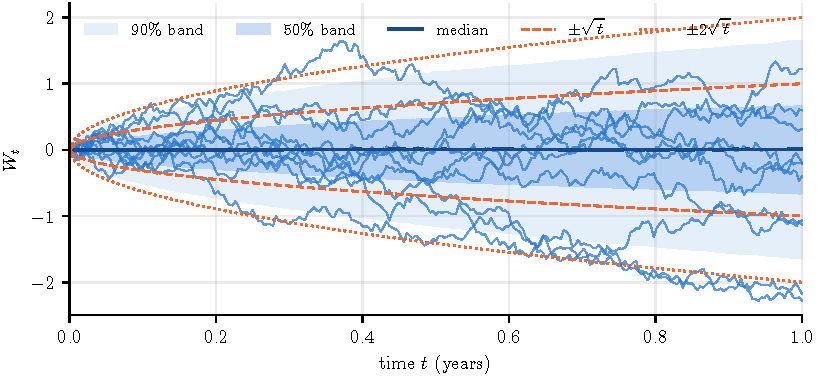
\includegraphics[width=\textwidth]{bm_paths}
\caption{Brownian motion. Ten sample paths (thin), the 50\% and 90\% bands across all paths,
and the curves $\pm\sqrt t$ and $\pm2\sqrt t$.}
\label{fig:bmpaths}
\end{figure}

Figure~\ref{fig:bmchecks} tests the definition. Panel (a) matches the histogram of $W_1$ to the
$N(0,1)$ density. Panel (b) shows the sample variance across paths lying on the line $t$. Panel
(c) takes one path on $2^{16}$ steps and computes both variations on coarser and finer grids. The
sum of squared increments settles at $T=1$ (\QVFinest{} on the finest grid). The sum of absolute
increments keeps growing like $\sqrt n$ and reaches \TVFinest. This is the roughness described
in Section~\ref{sec:models}, seen on an actual path.

\begin{figure}[h]
\centering
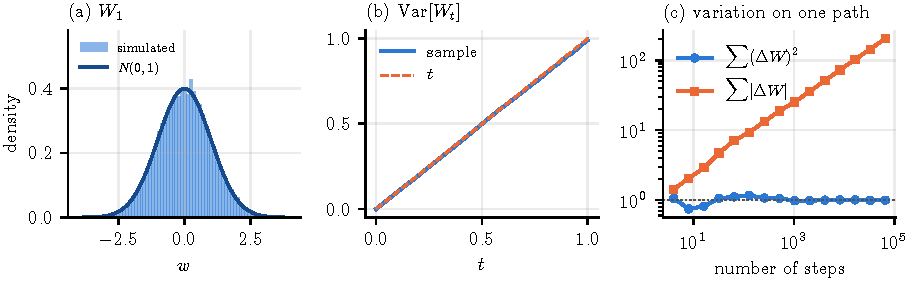
\includegraphics[width=\textwidth]{bm_checks}
\caption{(a) Distribution of $W_1$. (b) $\Var[W_t]$ across paths against $t$. (c) Quadratic
variation (blue) and total variation (orange) of one path as the grid is refined.}
\label{fig:bmchecks}
\end{figure}

\subsection{Geometric Brownian motion}

Figure~\ref{fig:gbmpaths} uses the same Brownian paths as Figure~\ref{fig:bmpaths}. The paths
stay positive and the bands are no longer symmetric: the upper band is wider than the lower one.
The terminal histogram in panel (b) is skewed to the right and lies on the lognormal density. The
mean of $S_1$ is $S_0e^{\mu}=\GBMMeanTh$, above the median $\GBMMedTh$. Across all paths $S_1$
ranges from \GBMMin{} to \GBMMax.

\begin{figure}[h]
\centering
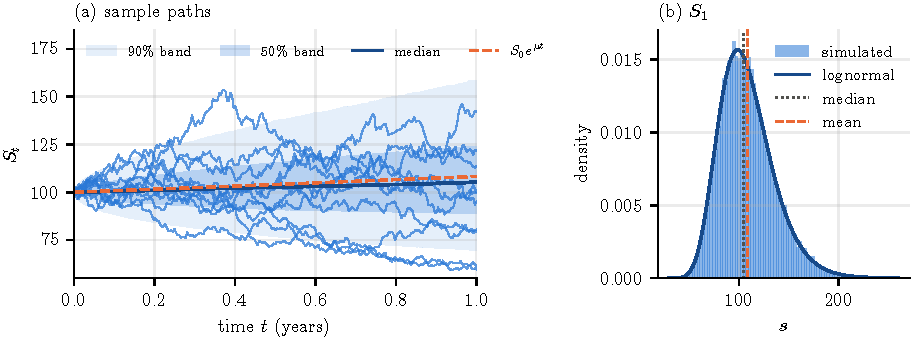
\includegraphics[width=\textwidth]{gbm_paths}
\caption{Geometric Brownian motion with $S_0=100$, $\mu=0.08$, $\sigma=0.25$. (a) Paths, bands,
median and the mean curve $S_0e^{\mu t}$. (b) Distribution of $S_1$ against the lognormal
density, with its mean and median.}
\label{fig:gbmpaths}
\end{figure}

Figure~\ref{fig:gbmsigma} changes only $\sigma$. In panel (a) one set of shocks drives three
prices: a larger $\sigma$ gives larger swings in both directions. Panel (b) shows the effect on
the distribution of $S_1$. All three densities have the same mean, $S_0e^\mu$, because $\sigma$
does not appear in $\E[S_t]$. The median, marked by a triangle, moves left as $\sigma$ grows.
The typical outcome gets worse while the average stays put, and the gap is paid for by a long
right tail. This is why a volatile asset with a high expected return can still lose money on
most paths.

\begin{figure}[h]
\centering
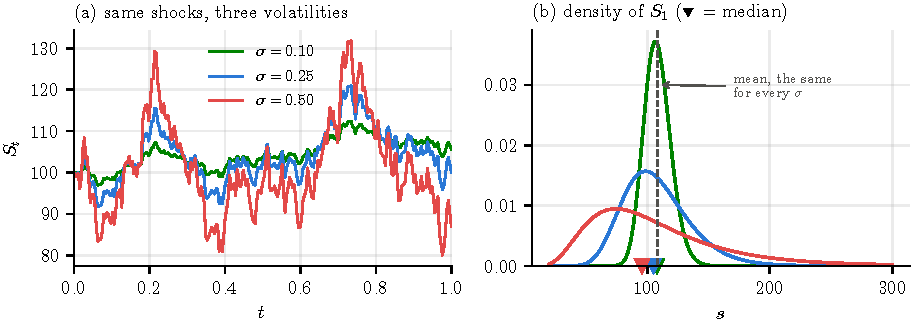
\includegraphics[width=\textwidth]{gbm_sigma}
\caption{Effect of volatility in GBM. (a) The same Brownian path with $\sigma=0.10$, $0.25$ and
$0.50$. (b) Lognormal densities of $S_1$; triangles mark the medians, the dashed line the common
mean.}
\label{fig:gbmsigma}
\end{figure}

Figure~\ref{fig:gbmerror} compares the two time-stepping schemes with the exact solution. On a
log-log scale the errors are straight lines. The fitted slopes are \EulerOrder{} for Euler and
\MilsteinOrder{} for Milstein, in line with the strong orders $1/2$ and $1$. Halving the step
cuts the Euler error by only about 30\%. The Milstein error halves.

\begin{figure}[h]
\centering
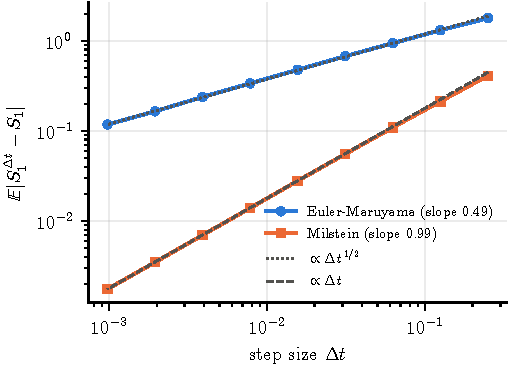
\includegraphics[width=0.6\textwidth]{gbm_error}
\caption{Strong error at $T=1$ of the Euler--Maruyama and Milstein schemes for GBM, against
the exact solution driven by the same shocks (5{,}000 paths). Grey lines show slopes $1/2$
and $1$.}
\label{fig:gbmerror}
\end{figure}

\subsection{The Ornstein--Uhlenbeck process}

Figure~\ref{fig:oupaths}(a) starts the OU process from $-1.5$, $0$ and $1.5$. Paths from all
three starting points end up in the same band around $\mu=0$, and the thick curves are the
theoretical means $\mu+(X_0-\mu)e^{-\theta t}$. With $\theta=2$ the half-life is
$\ln2/\theta=\OUHalfLife$. After about $1.5$ time units, four half-lives, less than $7\%$ of the
starting gap is left. Panel (b) shows the whole distribution of $X_t$ over time as a heat map,
built from all 20{,}000 paths started at $1.5$. It is narrow at the start, slides down toward
$0$, and stops widening once it reaches the stationary spread. The dashed lines are the mean
$\pm2$ standard deviations from \eqref{eq:oumom}, and they follow the edge of the dark region.

\begin{figure}[h]
\centering
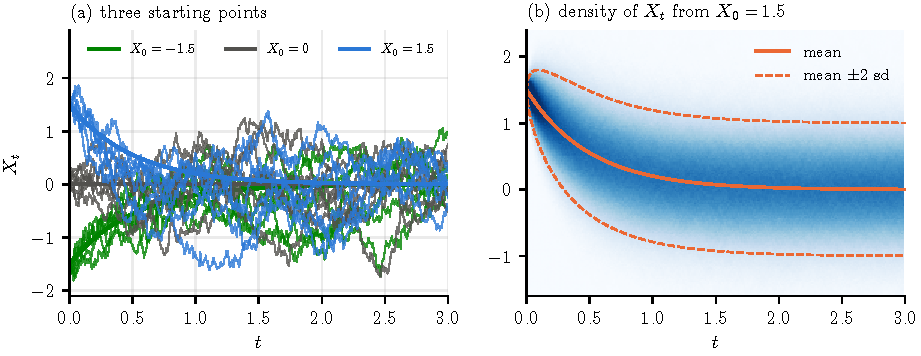
\includegraphics[width=\textwidth]{ou_paths}
\caption{OU process with $\theta=2$, $\mu=0$, $\sigma=1$. (a) Six paths from each of three
starting points, with the theoretical means. (b) Density of $X_t$ over time from $X_0=1.5$
(darker means more paths), with the mean and the mean $\pm 2$ standard deviations.}
\label{fig:oupaths}
\end{figure}

Figure~\ref{fig:oustat} looks at the long run. In panel (a) the distribution of $X_3$ matches
the stationary law $N(0,\sigma^2/2\theta)=N(0,0.25)$. In panel (b) we start paths from that law
and measure the correlation between $X_0$ and $X_\tau$. It decays as $e^{-\theta\tau}$, so the
process keeps a short memory. Panel (c) feeds the same shocks into three speeds of mean
reversion. A larger $\theta$ pulls the path to $0$ faster and keeps it in a narrower range,
since the stationary standard deviation is $\sigma/\sqrt{2\theta}$.

\begin{figure}[h]
\centering
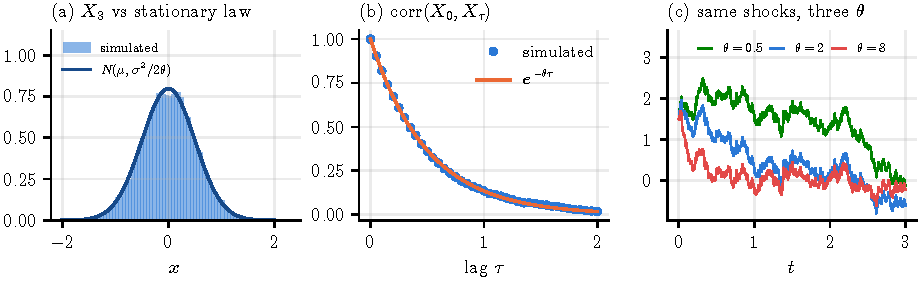
\includegraphics[width=\textwidth]{ou_stationary}
\caption{Long-run behaviour of the OU process. (a) $X_3$ against the stationary density.
(b) Autocorrelation under the stationary law. (c) One shock path with $\theta=0.5$, $2$ and $8$.}
\label{fig:oustat}
\end{figure}

\subsection{Short-rate models (VIR): Vasicek and CIR}

Figure~\ref{fig:rates} shows ten years of weekly short rates. Both models start at $2\%$ and
rise toward $5\%$ along the same mean curve. They spread differently. In Vasicek the noise has
the same size at every level, so the band is symmetric and part of it lies below zero. In CIR
the noise is proportional to $\sqrt{r_t}$. It is small when rates are low and large when they are
high, which gives a band squeezed at the bottom and stretched at the top. The lowest Vasicek
value across all paths and weeks is \VasMin\%. The lowest CIR value is \CIRMin\%.

\begin{figure}[h]
\centering
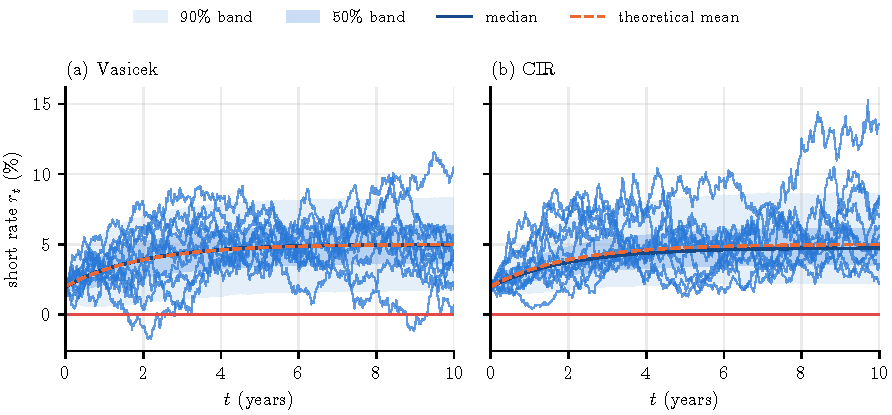
\includegraphics[width=\textwidth]{rate_paths}
\caption{Short rate over ten years under (a) Vasicek and (b) CIR, with the same mean and the
same long-run variance. The red line is zero.}
\label{fig:rates}
\end{figure}

Figure~\ref{fig:ratecompare}(a) puts the two ten-year distributions on top of each other. They
have the same mean and nearly the same variance, but Vasicek is a symmetric normal with a left
tail below zero, while CIR is skewed to the right and stops at zero. Panel (b) tracks
$\mathbb P(r_t<0)$. For Vasicek it climbs above $2\%$ in the first two years, while the rate is
still near its low starting point and the variance is growing. It then settles near its
long-run value $\Phi(-b/\sqrt{\sigma^2/2a})$. At ten years the formula gives \PNegTh\% and the
simulation \PNegSim\%. Looked at path by path, \PNegEver\% of Vasicek paths dip below zero at
least once in the ten years. No CIR path does.

Panel (c) plots yield curves from the bond formulas \eqref{eq:vasbond} and \eqref{eq:cirbond}
for three starting rates, with the Monte Carlo prices from our paths as markers. Starting below
$b$ gives a rising curve, and starting above $b$ gives a falling one. At $r_0=b$ the curve bends
slightly down toward its long-run limit $b-\sigma^2/2a^2=\YInf\%$, because uncertainty about
future rates raises bond prices and lowers yields. The simulated yields lie on the formula, and
the Vasicek and CIR curves almost coincide. For pricing bonds the two models agree. Where they
differ is the left tail of the rate itself.

\begin{figure}[h]
\centering
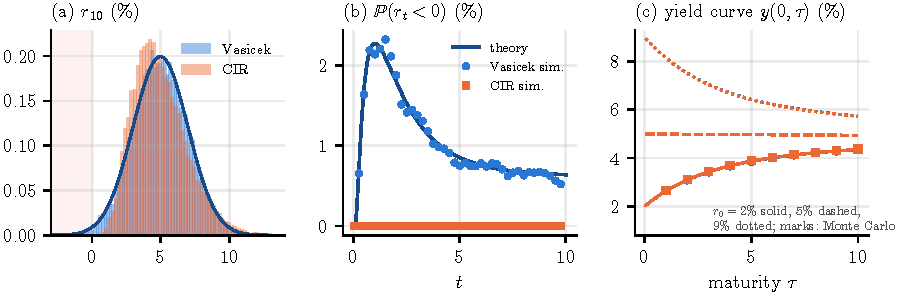
\includegraphics[width=\textwidth]{rate_compare}
\caption{Vasicek (blue) and CIR (orange). (a) Distribution of $r_{10}$; the line is the
Vasicek normal density and the shaded area is below zero. (b) Probability of a negative rate
over time. (c) Yield curves from the closed forms for $r_0=2\%$, $5\%$, $9\%$; markers are
Monte Carlo yields for $r_0=2\%$.}
\label{fig:ratecompare}
\end{figure}

\subsection{Accuracy}

Table~\ref{tab:moments} lists every check. Each simulated value is within \MaxZ{} standard
errors of its formula. With \NChecks{} checks, a largest $|z|$ of about $2$ is what pure chance
would produce, so the table shows no sign of bias. The bond prices are included even though they
carry the trapezoid error from Section~\ref{sec:method}, and they pass too.

\begin{table}[h]
\centering\small
\caption{Simulated values against closed-form values. SE is the Monte Carlo standard error and
$z=(\text{simulated}-\text{theory})/\text{SE}$.}
\label{tab:moments}
\begin{tabular}{@{}llrrrr@{}}
\toprule
Model & Quantity & Theory & Simulated & SE & $z$ \\
\midrule
BM & $\mathbb{E}[W_1]$ & $0$ & $0.0041667$ & $0.007$ & $+0.59$ \\
 & $\mathrm{Var}[W_1]$ & $1$ & $0.99135$ & $0.0099$ & $-0.87$ \\
 & $\mathbb{E}[W_{1/2}W_1]=\min(s,t)$ & $0.5$ & $0.49382$ & $0.0061$ & $-1.02$ \\
\midrule
GBM & $\mathbb{E}[S_1]$ & $108.33$ & $108.41$ & $0.19$ & $+0.40$ \\
 & $\mathrm{Var}[S_1]$ & $756.85$ & $746.77$ & $9$ & $-1.12$ \\
 & $\mathbb{P}(S_1\le \mathrm{median})$ & $0.5$ & $0.494$ & $0.0035$ & $-1.70$ \\
 & $\mathbb{E}[\ln S_1]$ & $4.6539$ & $4.655$ & $0.0018$ & $+0.59$ \\
\midrule
OU & $\mathbb{E}[X_1]$ & $0.203$ & $0.20342$ & $0.0035$ & $+0.12$ \\
 & $\mathrm{Var}[X_1]$ & $0.24542$ & $0.24465$ & $0.0024$ & $-0.32$ \\
 & $\mathrm{Var}[X_3]$ (near $\sigma^2/2\theta$) & $0.25$ & $0.24976$ & $0.0025$ & $-0.10$ \\
\midrule
Vasicek & $\mathbb{E}[r_1]$ & $0.031804$ & $0.031883$ & $0.00011$ & $+0.70$ \\
 & $\mathrm{Var}[r_1]$ & $0.00025285$ & $0.00024979$ & $2.5\times10^{-6}$ & $-1.24$ \\
 & $P(0,5)$ & $0.82443$ & $0.82419$ & $0.00036$ & $-0.65$ \\
 & $P(0,10)$ & $0.64741$ & $0.64694$ & $0.00049$ & $-0.95$ \\
 & $\mathbb{P}(r_{10}<0)$ & $0.0063881$ & $0.00575$ & $0.00053$ & $-1.19$ \\
\midrule
CIR & $\mathbb{E}[r_1]$ & $0.031804$ & $0.031875$ & $8.3\times10^{-5}$ & $+0.85$ \\
 & $\mathrm{Var}[r_1]$ & $0.0001383$ & $0.00013876$ & $1.7\times10^{-6}$ & $+0.28$ \\
 & $P(0,5)$ & $0.82395$ & $0.82347$ & $0.00029$ & $-1.65$ \\
 & $P(0,10)$ & $0.64676$ & $0.64596$ & $0.00043$ & $-1.86$ \\
\bottomrule

\end{tabular}
\end{table}

%=====================================================================
\section{Conclusion}
\label{sec:conclusion}

We simulated Brownian motion, geometric Brownian motion, the Ornstein--Uhlenbeck process and
the Vasicek and CIR short-rate models from their exact transition laws, and every simulated
quantity agrees with its formula within Monte Carlo error. The simulations make the differences
between the models easy to see. Brownian motion and GBM have no level to return to, and their
spread grows without bound. GBM stays positive, but its median drifts below its mean as
volatility rises. The OU process and the two rate models settle into a stationary band, and the
OU process loses track of where it started within a few half-lives. Among the rate models,
Vasicek and CIR give almost the same bond prices, but only CIR keeps the rate positive. Vasicek
allows negative rates on about a quarter of the paths over ten years.

Exact simulation was possible here because each model has a closed-form transition law. For
models without one, a scheme such as Euler or Milstein is needed. Our GBM test shows the cost:
Euler converges at order $1/2$, so it needs about four times as many steps to halve its error.

\bibliographystyle{plain}
\bibliography{refs}

\appendix
\section{Code}
The script below produces every figure and every number in this report
(\texttt{uv run --with numpy --with matplotlib python sim.py}).
\lstinputlisting[language=Python]{sim.py}

\end{document}
